\documentclass[landscape, a4paper]{article}
\usepackage[margin=0cm,top=0.4cm,bottom=0.4cm,left=0.4cm,right=0.4cm]{geometry}
% \usepackage[showframe,margin=0cm,top=0.5cm,bottom=0.5cm,left=0.5cm,right=0.5cm]{geometry}
\usepackage[export]{adjustbox}
\usepackage{ipsum}
\usepackage{xcolor}
\usepackage{caption}
\usepackage{csquotes}
\usepackage[parfill]{parskip}

\captionsetup{labelformat=empty, justification=centering, font={color=PrimaryColor}}

\definecolor{PrimaryColor}{HTML}{8FA85F}
\newcommand\alert[1]{\textcolor{PrimaryColor}{\textbf{#1}}}

\begin{document}
\noindent
\centering
\footnotesize
\begin{minipage}[t]{0.31\textwidth}
	\setlength{\parskip}{0.25cm}

	\vspace{0.5cm}

		\textcolor{PrimaryColor}{
			\rule{\linewidth}{0.5mm}
			\vspace{-0.1cm}
			\begin{center}
				\large
				\textsc{Hike to the Kybfelsen castle ruin}
			\end{center}
			\rule{\linewidth}{0.5mm}
		}

    An unforgettable hike through the enchanting natural landscape of Freiburg's \alert{Günterstal}, up to the mysterious castle ruins of Kybfelsen! The path leads deep into the forest, past babbling brooks, imposing rocks, and magical clearings. After just a few steps, you are immersed in the peaceful silence of the Black Forest, where you are enveloped by towering trees and swallowed by the woods, escaping the hustle and bustle of the big city.

    The \alert{Arboretum in Günterstal} invites you on a journey through the world of trees. A selection of planted trees and shrubs has been organized by theme and equipped with informational signs. Each of the five themed trails is dedicated to a region of origin, a group of related tree species, or a special aspect of the relationships between the world of trees and the world of animals or humans.
    Many of the trees here are botanical treasures, including living fossils like the ginkgo and ancient conifers that have survived since the time of the dinosaurs. With over 1,300 species, the Arboretum is one of the most diverse collections of its kind in Germany.
    % It also includes unique paths such as the \enquote{WaldMenschen} sculpture trail and the \enquote{Mycelium} trail, which explores the underground world of fungi and forest ecosystems.

		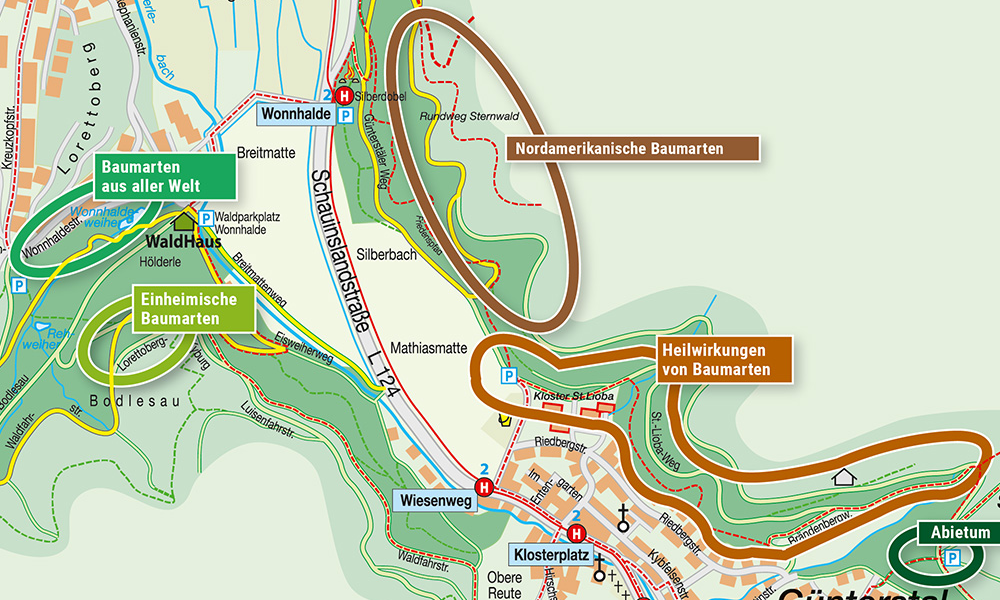
\includegraphics[width=\linewidth]{./figures/arboretum.png}
		\captionof{figure}{Arboretum in Günterstal with its themed trails}
		\setlength{\parskip}{0.25cm}

    An \alert{arboretum} (Latin, a variant of arbustum, here specifically in the sense of tree planting, from arbor meaning tree) is a collection of various, often exotic woody plants (not grown in containers); this can be, for example, a botanical garden in which primarily trees and shrubs are planted. If only shrubs are planted, it is referred to as a fruticetum. If only coniferous trees are planted in an arboretum, it is called a pinetum.

\end{minipage}%
\hfill%
\vrule width 0.01cm
\hfill%
\begin{minipage}[t]{0.31\textwidth}
	\setlength{\parskip}{0.25cm}
  The \alert{Stadtwald Arboretum} was established as early as the late 19th century, when Freiburg's foresters began planting exotic tree species in nearby forests for experimental purposes. However, only a few tree species were successfully integrated into the native forest ecosystem. The most famous and characteristic example for Freiburg's Stadtwald is the forestry use of the North American tree species Douglas fir, which has been used in forestry in Freiburg since 1896 and is now one of the most economically important tree species.

	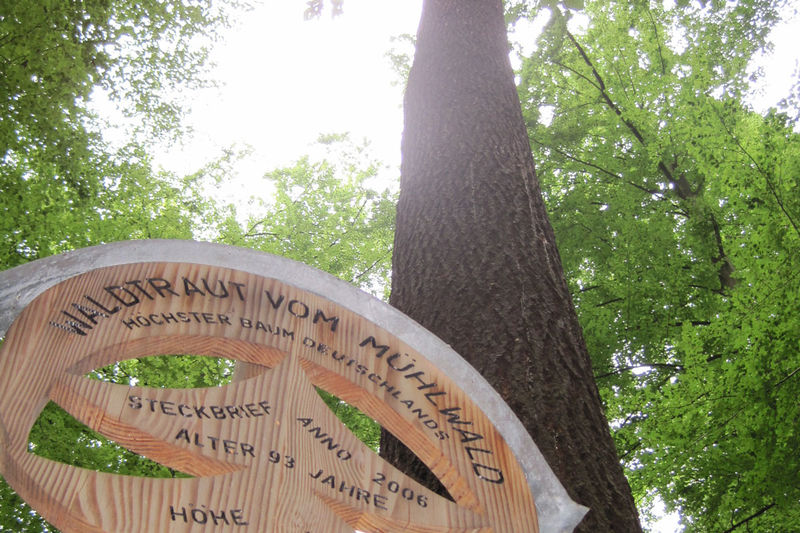
\includegraphics[width=\linewidth]{./figures/waldraud.png}
	\captionof{figure}{Waldtraut of the Mühlwald, the tallest officially measured tree in Germany}
	\setlength{\parskip}{0.25cm}

  The \alert{Douglas fir} is economically significant in the Black Forest because it grows quickly, is resistant to drought and pests, and provides high-quality wood that can be used in a variety of ways. Additionally, as part of mixed forests, it improves the stability and resilience of the forest, making it especially attractive in the face of climate change.\\
By the way, the name Douglas fir has nothing to do with the perfume and cosmetics company Douglas. The name of the Douglas fir comes from the Scottish botanist David Douglas, who brought the tree species from North America to Europe in the 19th century. The name of the company Douglas, on the other hand, goes back to the founder John Sharp Douglas, who opened a soap factory in Hamburg in 1821, which later became a perfume and cosmetics company.

  A special highlight along the route is \alert{Waldtraud}, the (in the year 2025) 115-year-old Douglas fir, which, with its proud height of 67 meters, holds the title of tallest tree in Germany. It was planted in 1913 as a three-year-old tree at its current location, slightly south of today's Freiburg-Günterstal Arboretum.

However, the hiking route has even more to offer: at several viewpoints, you can enjoy breathtaking views over Freiburg and Günterstal. In addition to the landscape, you also experience a piece of history, many famous personalities have left their mark here.

\end{minipage}%
\hfill\color{white}%
\vrule width 0.01cm
\hfill\color{black}%
\begin{minipage}[t]{0.31\textwidth}
	\setlength{\parskip}{0.25cm}

  \alert{Günterstal} is mentioned by name for the first time in a deed of ownership from the year 804, at that time as \enquote{Gundherrerhusir} (houses of Günther) in the Mark of Merzhausen. Around 300 years later, the place appears again under the name \enquote{Guntheristal}. Around 1221, a nobleman, who according to an 18th-century tradition was named Günther von Kibenfels, gave the land in Günterstal to his daughter Adelheid. There, she and her companions built a small monastic complex. In a document from 1224, the monastery in \enquote{Günterstal} is mentioned for the first time. However, Günther von Kibenfels cannot be the namesake of the place, since the name \enquote{Günter} had already appeared much earlier in the place name. Along the hiking route, you also pass the gatehouse of the former monastery, which is crossed by the streetcar.

  Among others, the prominent German mathematician \alert{Ernst Zermelo} is buried in the cemetery in Günterstal in Freiburg. His grave lies next to that of Edmund Husserl. Ernst Zermelo was a significant mathematician who revolutionized set theory. He formulated the Zermelo axiom system, which forms the foundation of modern set theory. Particularly well-known are the \alert{Zermelo-Fraenkel axioms}, which precisely define the mathematical structure of sets and are widely used in mathematics today. Another important result of his work is the Axiom of Choice, which is essential in many areas of mathematics, such as analysis and algebra. Zermelo's contributions laid the foundation for many modern mathematical theories.

	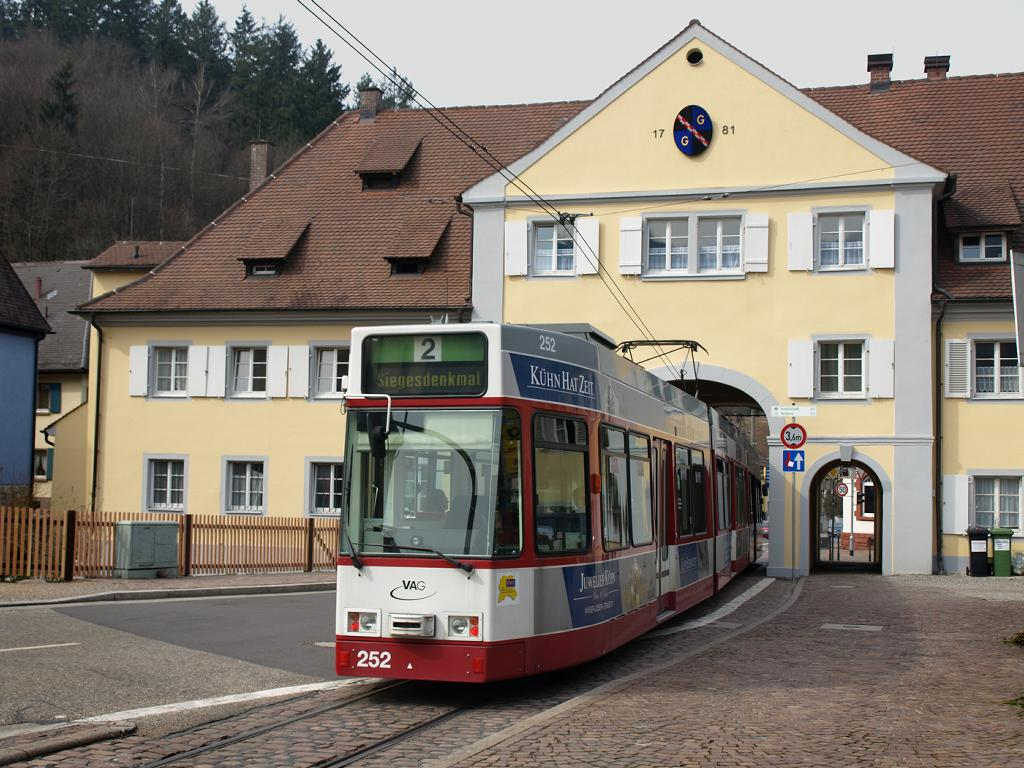
\includegraphics[width=\linewidth]{./figures/tor.png}
	\captionof{figure}{Gatehouse of the former monastery}
	\setlength{\parskip}{0.25cm}

  Starting in 1926, he held an honorary professorship at the \alert{Albert-Ludwigs-Universität} in Freiburg im Breisgau, but had to give up this position in 1935 because he refused to begin his lectures with the Hitler salute, which was reported by colleagues (Gustav Doetsch and his assistant Eugen Schlotter). After the Second World War, he resumed his position as honorary professor, but due to his health condition, he was no longer able to give lectures.

\end{minipage}%
\newpage
\begin{minipage}[t]{0.31\textwidth}
	\vspace{0cm}
	\setlength{\parskip}{0.25cm}

	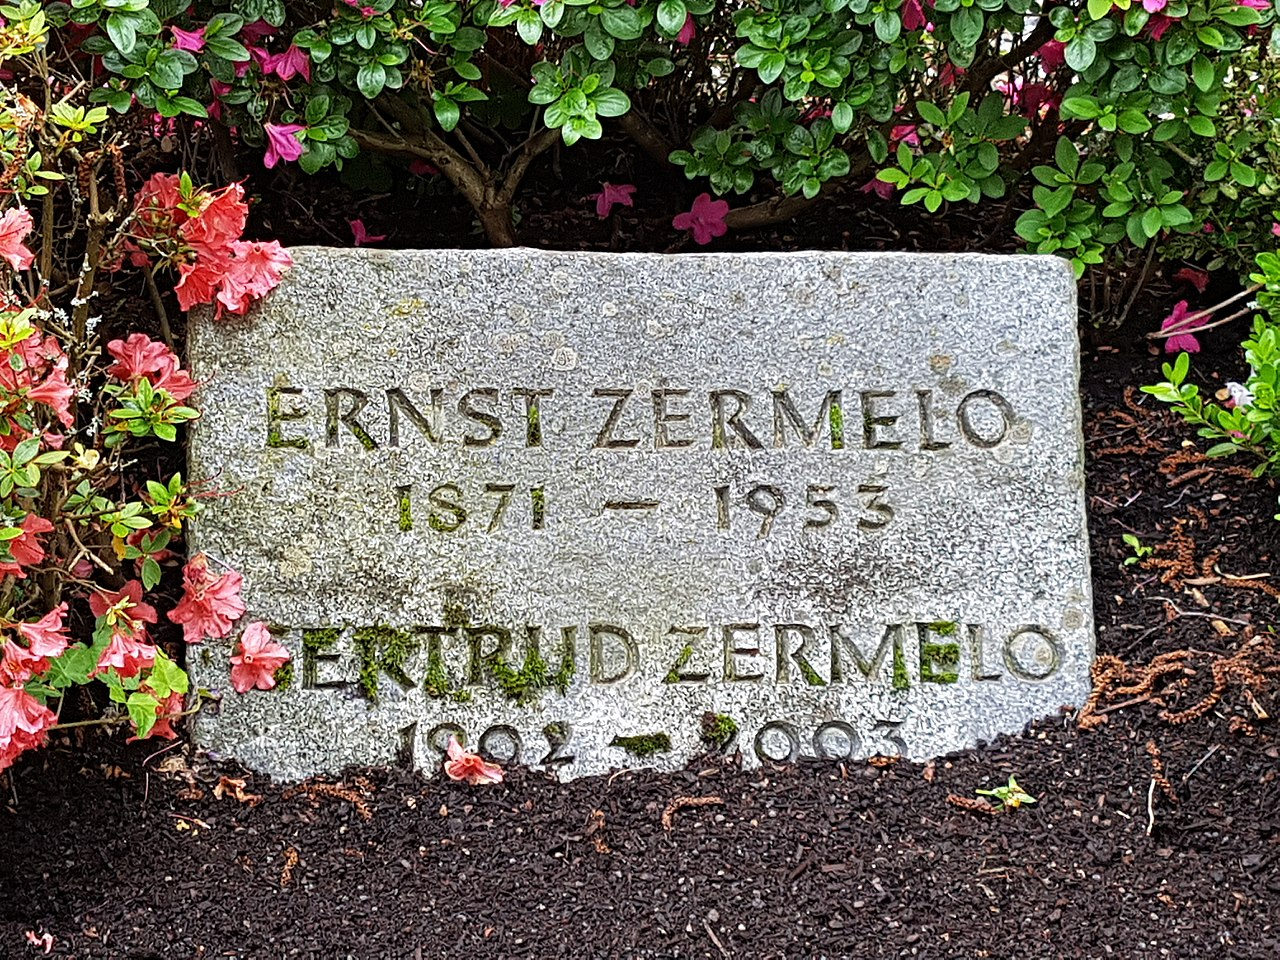
\includegraphics[width=\linewidth]{./figures/grabstein.png}
	\captionof{figure}{Gravestone of Ernst Zermelo in the Günterstal cemetery}
	\setlength{\parskip}{0.25cm}

  In April 2018, the Eckerstraße in Freiburg, where the Mathematical Institute of the Albert-Ludwigs-Universität Freiburg is located, was renamed \alert{Ernst-Zermelo-Straße} in his honor. As the explanatory sign beneath the new name states, the street was renamed due to the problematic pioneering role of Alexander Ecker as a nationalist racial ideologist. The new name is well chosen for the institute: Ernst Zermelo is the namesake of the home address of the Ernst Mach Institute and the mathematics education department of the University of Freiburg, both are institutions that likely would not get far without Zermelo's set theory. % Even a celestial body, the asteroid 14990 Zermelo, is named after the mathematician.


	\includegraphics[width=\linewidth]{./figures/straßenschild.png}
	\captionof{figure}{Former Eckerstraße renamed to Ernst-Zermelo-Straße}
	\setlength{\parskip}{0.25cm}
\end{minipage}%
\hfill%
\vrule width 0.01cm
\hfill%
\begin{minipage}[t]{0.31\textwidth}
	\setlength{\parskip}{0.25cm}
	\vspace{0cm}

  Along the hiking route, you come to castle ruin \alert{Kybfelsen}, which lies mysteriously hidden among the trees. A castle on the Kybfelsen is mentioned in the chronicle of Matthias of Neuenburg from the mid-14th century. The name \enquote{Kyburg} first appears in 1484 in the legal code of Kappel. Excavation findings at the castle site in the 1920s by Otto Kantorowicz confirm the existence of the structure already during the rule of the Zähringer dynasty in the Breisgau in the late 11th or early 12th century. % Finds of reading ceramics, which can be dated to the 12th and early 13th centuries, complete the picture of the period during which the fortified site was in use.

The \alert{district of Zähringen} in Freiburg is named after the Zähringer dynasty, a noble family that played a significant role in the region during the Middle Ages. The name \enquote{Zähringen} is derived from the former Zähringen Castle, which was built in the 11th century by the Zähringer. This castle was located near today’s Zähringen district and served as a strategically important point to control the surrounding area. Zähringerstraße and Zähringen Castle still bear witness to this history.

The \alert{Zähringen Castle} on the Schlossberg lost its importance in the 13th century and was later destroyed. Today, only a few remnants of the castle remain. The ruins are located on the Zähringen Hill in the Zähringen district, where the foundations and parts of the former castle complex can still be seen.

	\includegraphics[width=\linewidth]{./figures/kybfelsen.png}
	\captionof{figure}{The castle ruins of Kybfelsen}
	\setlength{\parskip}{0.25cm}

  The \alert{Zähringer} were an important Swabian princely dynasty of the Middle Ages that played a decisive role in the founding and development of Freiburg im Breisgau. Duke Conrad of Zähringen founded the city in 1120 as a market town by establishing a market and allocating plots to merchants. The Zähringer built a castle on the Schlossberg in 1091, which significantly promoted the city's development. They granted Freiburg extensive freedoms and privileges, turning the city into the center of their dominion. These measures helped to advance trade and the economic development of the region. After the extinction of the Zähringer line in 1218, Freiburg passed to the Counts of Urach, who from then on called themselves Counts of Freiburg. Nevertheless, the positive memory of the Zähringer as founders and patrons of the city remained alive in Freiburg. Their legacy left a lasting mark on the development of the city and the entire region between the Black Forest and Lake Geneva.

	% 1080 wurde in einem Bericht Otto von Freisings erstmals eine Burg Zähringen erwähnt, ein erster urkundlicher Nachweis befindet sich im Rotulus Sanpetrinus von 1128. Die Entstehungsgeschichte der Burg liegt im Dunkeln. Das darunterliegende Dorf Zähringen wurde 1008 erstmals in einer Schenkungsurkunde, der sogenannten Wildbannurkunde von König Heinrich II. an das Bistum Basel erwähnt, zusammen mit den Namen der Freiburger Stadtteile Herdern und Wiehre, der Nachbargemeinde Gundelfingen und anderer Orte im Breisgau.
\end{minipage}%
\hfill\color{white}%
\vrule width 0.01cm
\hfill\color{black}%
\begin{minipage}[t]{0.31\textwidth}
	\vspace{0cm}
	\setlength{\parskip}{0.25cm}

	% Ein kulinarischer Höhepunkt erwartet einen im \alert{Waldrestaurant St. Valentin}, wo regionale Spezialitäten und kühle Getränke zur Stärkung erworben werden können. \alert{St. Valentin} war ein christlicher Märtyrer aus dem 3. Jahrhundert, von dem es mehrere Überlieferungen gibt, darunter als ein Priester in Rom und ein Bischof in Terni. Er wird oft mit heimlichen Eheschließungen in Verbindung gebracht, was zu seiner späteren Hinrichtung führte. Die Assoziation mit dem Valentinstag und der Liebe entstand jedoch erst im Mittelalter und basiert mehr auf romantischen Traditionen als auf historischen Tatsachen.
  A culinary highlight awaits you at the \alert{Waldrestaurant St. Valentin}, where regional specialties and cool drinks can be enjoyed for refreshment. \alert{St. Valentin} was a Christian martyr from the 3rd century, about whom there are several accounts, including one as a priest in Rome and another as a bishop in Terni. He is often associated with performing secret marriages, which ultimately led to his execution. However, the association with Valentine's Day and love only emerged in the Middle Ages and is based more on romantic traditions than on historical facts.

	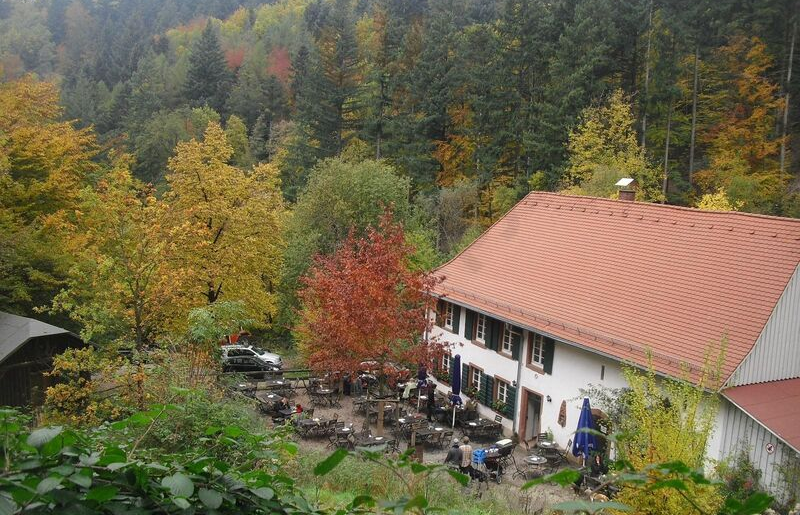
\includegraphics[width=\linewidth]{./figures/stvalentin_2.png}
	\captionof{figure}{Waldrestaurant St. Valentin from a bird’s-eye view}
	\setlength{\parskip}{0.25cm}

  Echoing the legacy of Roman architectural influence, the \alert{St. Lioba Monastery} in Freiburg Günterstal is housed in a Tuscan-style villa that was established in 1927. Tuscan style is a classical architectural tradition from central Italy, rooted in Roman and Renaissance design, featuring symmetry, earthy materials, and terracotta. Terracotta is a type of baked clay that’s been used for thousands of years in art, architecture, and construction. \alert{St. Lioba} (c. 710–782) was an English nun and missionary. She helped spread Christianity in what is now Germany.

  % The Freiburg district of \alert{St. Georgen} owes its name, by the way, to another Christian saint, Saint George. The name most likely derives from an early chapel or church that was dedicated to Saint George, as this saint was considered an important patron in the Middle Ages. At that time, it was common to name settlements after saints who served as patrons for the region and represented God's protection and blessing for the community.

% \alert{Saint George} was a Roman soldier and martyr of the 3rd century who died for his Christian faith. George was persecuted because of his Christian beliefs and was eventually martyred during the Diocletianic Persecution (around 303 AD) in Lydda (in present-day Israel). Because he refused to renounce his Christian faith and make sacrifices to the Roman gods, he was tortured and eventually beheaded. According to legend, he slew a dragon and thus saved a city, with the dragon legend symbolizing his role as a defender of good and of the Christian faith. As a patron saint of many countries and professions, especially knights and soldiers, he stands for courage, steadfastness, and commitment to faith.

  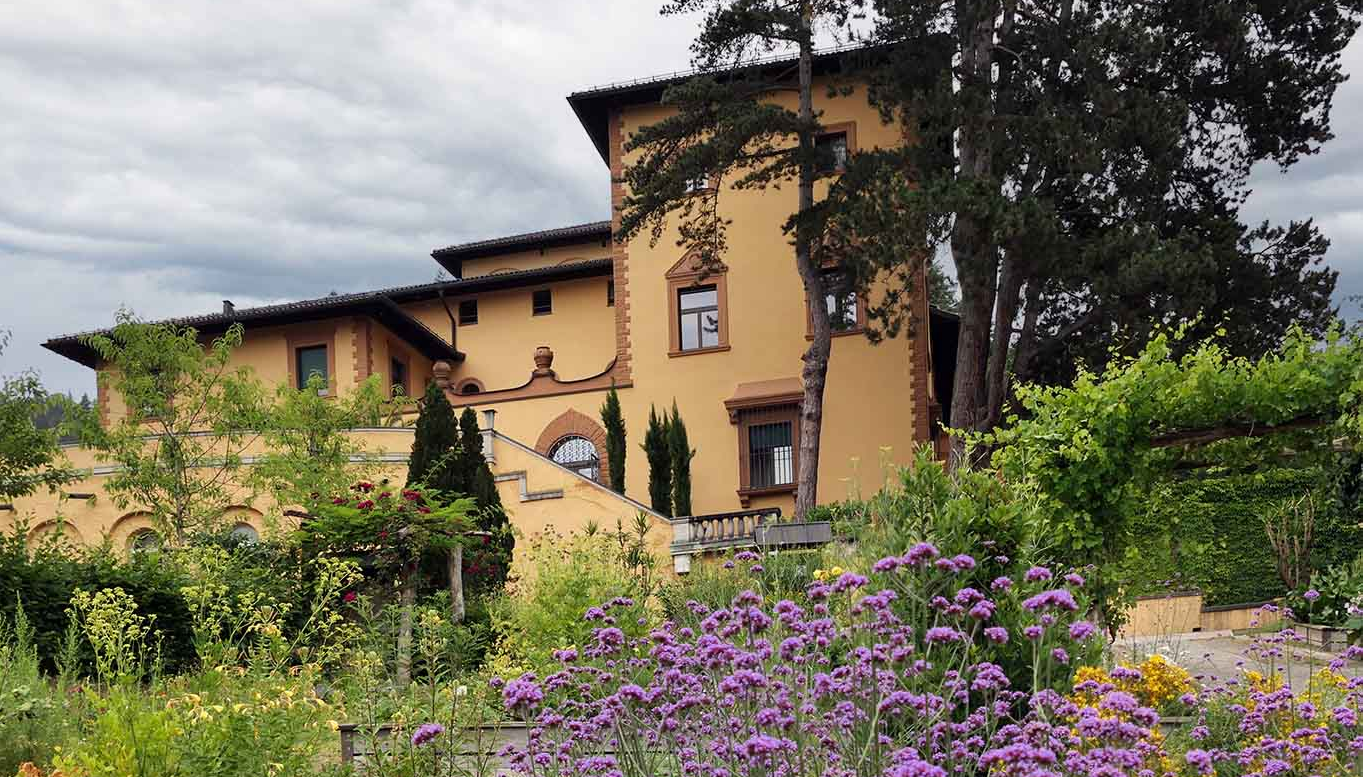
\includegraphics[width=\linewidth]{./figures/kloster_st_lioba.png}
	\captionof{figure}{St. Lioba Monastery, where Roman architecture lives on}
	\setlength{\parskip}{0.25cm}

\end{minipage}%
\end{document}
